\section{What is a project?}
\begin{itemize}
    \item A project is:
        \begin{itemize}
            \item A temporary endeavor undertaken to create a unique product, service or result. PMI definition.
            \item It has a determined start and end date.
            \item It is not a business process that is ongoing but rather have a specific expiring date.
            \item It is time bound and has a goal.
            \item The goal can be a result, service or produt.
            \item The output + the work employed to create it is called a scope. 
        \end{itemize}
    
    \item Elements of a project:
        \begin{itemize}
            \item Time (start and end date) + goal (product, service or result) + cost.
                \begin{figure}[H]
                    \centering
                    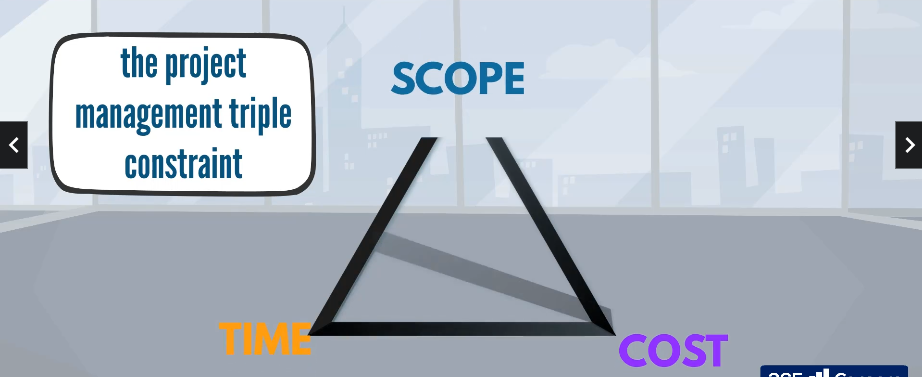
\includegraphics[width=\width\textwidth]{./figs/2022-10-20-14-09-12.png}
                    %\caption{}
                \end{figure}
            
            \item These three elements form what is known as a project management triangle where any change in one of the dimentions results in the changing of all the other dimensions, there is a tradeoff between these dimensions, when you want less time this might affect cost, etcetera.
        \end{itemize}
    
    \item Ending definition:
        \begin{itemize}
            \item A project is a temporary initiative that is agreed, planned, and executed to achive a specific goal.
            \item Projects are complex initiatives.
        \end{itemize}
\end{itemize}

%%%%%%%%%%%%%%%%%%%%%%%%%%%%%%%%%%%%%%%%%%%%%%%%%%%%%%
\section{Why do companies execute projects?}
\begin{itemize}
    \item All companies have goals. Some goals are for daily work goals and other goals are strategic.
    \item To achieve the strategic goals a company cannot lean on the same old strategies but rather create something new.
    \item In the implementation of any strategic goal you need to achieve in a company, you must do it usign a project. This is why companies execute projects. 
    \item In order to achieve the project as an output you need to put in the following inputs:
        \begin{itemize}
            \item Resources,
            \item Financial Resources, 
            \item Organizational resources, and
            \item Time.
        \end{itemize}
    
    \item In highly innovative indutries failing to prioritize getting the necessary resources in the right time might put the company at a significant disadvantage.
    \item Correct project management derives the following benefits:
        \begin{itemize}
            \item Financial, operational, customer related, non-profit.
        \end{itemize}
    
    \item Let's see the life cycle of a project:
        \begin{figure}[H]
            \centering
            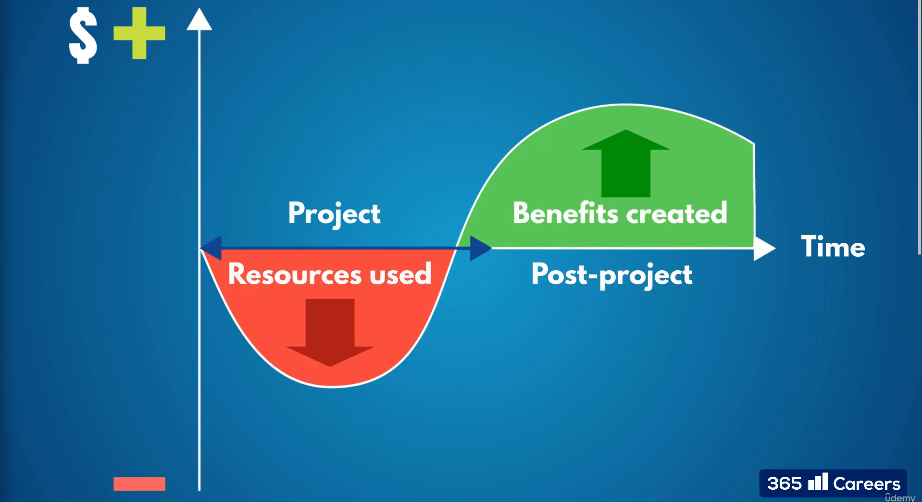
\includegraphics[width=\width\textwidth]{./figs/2022-10-20-14-19-00.png}
            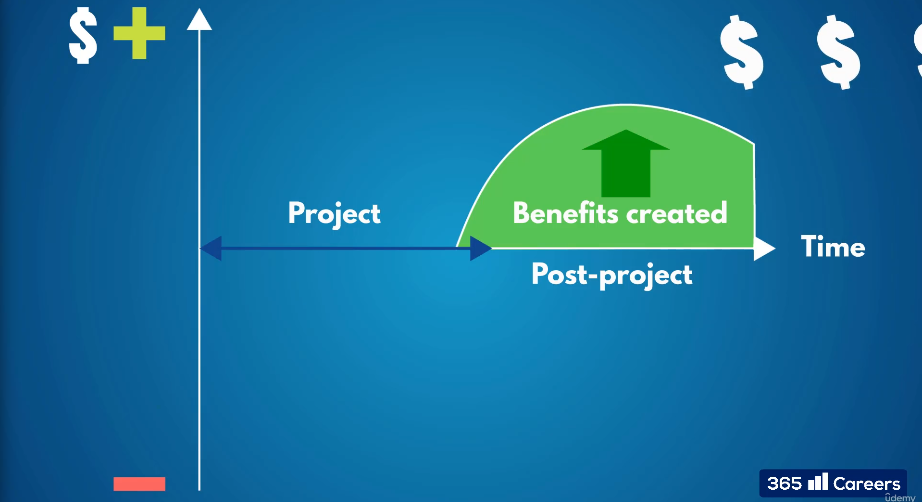
\includegraphics[width=\width\textwidth]{./figs/2022-10-20-14-19-22.png}
            %\caption{}
        \end{figure}
\end{itemize}

%%%%%%%%%%%%%%%%%%%%%%%%%%%%%%%%%%%%%%%%%%%%%%%%%%%%%%
\section{What creates the demand for a project? Prioritizing and selecting a project.}
\begin{itemize}
    \item A project must relate to a business strategy. So what creates the demand for a project in the first place.
    \item The following:
        \begin{itemize}
            \item Market need, to keep up or have advantage over the competition.
            \item Business need.
            \item Technological advancement. i.e. for example: automation.
            \item Customer request. i.e. satisfying client's needs.
            \item Legal requirements. For example: social media.
            \item Social needs. For example: building a bridge.
            \item Ecological impact considerations. For example: improving cars 
        \end{itemize}
    
    \item Once a specific goal arises, the PROJECT will be the instrument to achieve that goal.
\end{itemize}


\subsection{Priritizing and project selection}
\begin{itemize}
    \item The needs most likely will never arive one by one, so how do you choose which ones to do and in what order?
    \item This is when prioritizing comes in.
    \item The process is the following:
        \begin{itemize}
            \item First the project owner will propose the project via a project proposal to management to make it compete for the resources of the organization.
            \item Management will decide which project will be discarded, prioritized, or posponed for a later date.
            \item Prioritizing urgency: for example if some law requires some inmediate project or else they wont be able to operate, management will prioritize it because it is urgent.
            \item This is known as project selection.
        \end{itemize}
    
    \item The project selection process selects the order in which each project will be done, and will schedule the order in dates. Which projects will be concurrent etcetera. Management will make what is called a project portfolio, this is a document that contains the details on which projects will be done and in what order, and which project will be done at the same time (concurrently).
    \item Project Portfolio Management: the process of creating and managing the project portfolio in such a way that it uses the organization's resources in an optimal way.
    \item Projects are investments and need to be done in as efficient a manner as possible. Projects consume a lot of resources, finances, time, effort, attention, care, etcetera. If they are not aligned and optimized it may result in the organization's bankrupcy or at best to disapointed stakeholders.
\end{itemize}

%%%%%%%%%%%%%%%%%%%%%%%%%%%%%%%%%%%%%%%%%%%%%%%%%%%%%%
\section{What is a project manager? What is their commitment to a project?}
\begin{itemize}
    \item The project manager is the one responsable for the project, the PM is the CEO of the project. 
    \item The PM person needs to work between these constraints (budget, time, performance) in order to meet the goal and add value to the business.
        \begin{figure}[H]
            \centering
            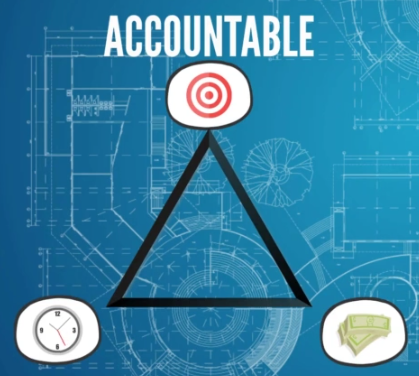
\includegraphics[width=\width\textwidth]{./figs/2022-10-20-20-42-25.png}
            %\caption{}
        \end{figure}
    
    \item This is a big responsability. The PM must therefore choose realistic projects, taking into account all costs, all time constraints. Otherwise they will not be able to delive and will be in problems. 
    \item It is a project manager's duty to do the following to a project:
        \begin{itemize}
            \item Asses, Discuss, Negotiatite, Adjust: demonstrate why the project will be ready in the proposed date, why it will cost the proposed amount. Otherwise refuse to take a project on.
        \end{itemize}
    
    \item What does it mean to be accountable?
        \begin{itemize}
            \item The project manager has the ultimate responsability, they can't blame the failure of a project on any one else. 'The buck stops with them'.
            \item Project manager must commit and deliver.
        \end{itemize}
    
    \item The PM responsability is not only responsable for themselves but also for the actions of their team members. A PM must be able to have full control, and take inmediate action upon a problem arising.
\end{itemize}

%%%%%%%%%%%%%%%%%%%%%%%%%%%%%%%%%%%%%%%%%%%%%%%%%%%%%%
\section{What are the skills and the knowledge a PM must have?}
\begin{itemize}
    \item The PM is the face of the project.
    \item They are the point of contact of the team.
    \item Must mediate between team members.
    \item Successfully relate with team members with all levels of seniority.
    \item They are accounable to deliver the expectations.
    \item They must therefore have:
        \begin{itemize}
            \item Skills, knowledege, attitude, and experience.
        \end{itemize}
    
    \item The three major qualities of PM:
        \begin{enumerate}
            \item Technical skills and knowledge.
                \begin{itemize}
                    \item PM triple constraint.
                    \item Theoretical framework.
                    \item PM tools and documents.
                    \item Personal organization (ability to organize you own tasks).
                    \item Task management (ability to fulfill tasks, prioritize and manage tasks).
                    \item Critical thinking (tell which information is useful and which is not).
                    \item Efficient use of software tools for PM.
                \end{itemize}

            \item Interpersonal soft skills:
                \begin{itemize}
                    \item Each project is unique and must adapt to a new set of persons each time. 
                    \item They need communication skills (90\% of their time will be in communications).
                    \item Team management, being able to asses performance and output of the team, the PM needs to be able to articulate the project's needs and requirements, identify impediments and keep the team motivated.
                    \item Leadership, ability to influence people in the desired direction, capacity to mediate.
                    \item Social skills, ability to work with a lot of people.
                    \item Advice: never talk exclusively about the project, talk also about personal lives and hobbies, otherwise team members will associate you only to office work and you will not be able to influence and motivate them personally. Also be humorous, it relaxes people.
                \end{itemize}
            
            \item Industry experience: 
                \begin{itemize}
                    \item Does the PM needs to be an expert in the industry in which their project are taking place? it depends, knowledge always helps.
                    \item Being an expert in a field does not imply success in managing the project related to that field. It helps but in order to manage project effectively you need first and formost... project management skills. Industry expertise is a bonus most of the time.
                    \begin{figure}[H]
                        \centering
                        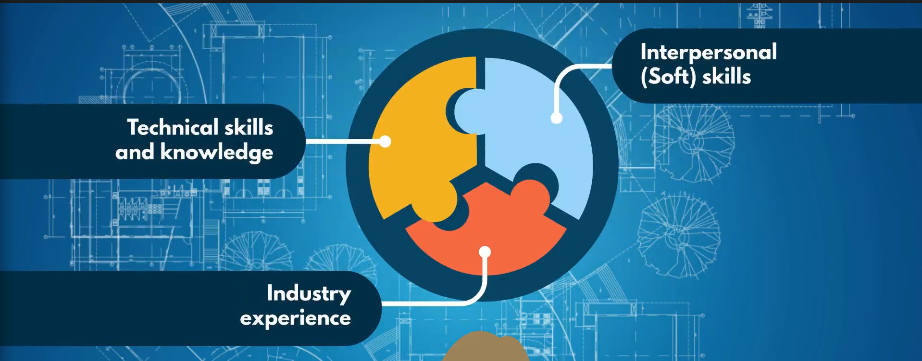
\includegraphics[width=\width\textwidth]{./figs/2022-10-20-21-01-29.png}
                        %\caption{}
                    \end{figure}
                \end{itemize}
        \end{enumerate}
\end{itemize}

%%%%%%%%%%%%%%%%%%%%%%%%%%%%%%%%%%%%%%%%%%%%%%%%%%%%%%
\section{Projects: a history lesson}
\begin{itemize}
    \item Project management has been going on for thousands of years. 
    \item An example includes the pyramids of ancient egypt. This construction was massive endeavor, involving materials and a workforce. The success of this most likely depended on good project management.
    \item Another example is when Columbus sailed to America, he did it with a budget of three ships and some ship crew and his proposal was rejected multiple times by various kings. Eventually they found a sponsor of this projects, the king and queen of Spain.
    \item Another example, 19th century and the industrial revolution, in which project management became more and more popular since more projects were going on.
    \item Another example, 20th century project management, the Gantt chart was created by Herny Gantt, it was used in WW1 to track and manage navy ship creation. 
        \begin{figure}[H]
            \centering
            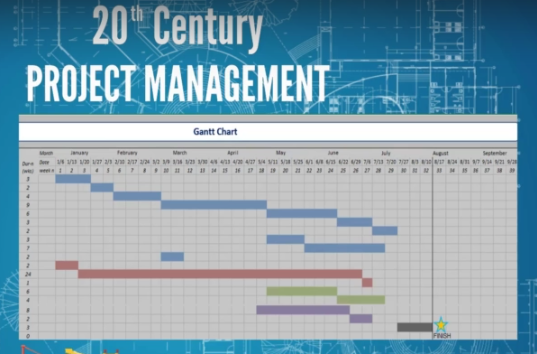
\includegraphics[width=\width\textwidth]{./figs/2022-10-20-21-23-46.png}
            %\caption{}
        \end{figure}
    
    \item In the late 1950s the \emph{critical path method} this is a methodology allows to calculate the fastest way to completing a project, finding links and connections between the activities involved.
    \item In the 1960s the Project management profession was established. The international project management association and project management institute established standards, best practices, tools and guidelines.
    \item The 21st century project management scheme is exceptional because the projects are incredibly complex and have many many variables and factors, as well as risks that must be all individually considered. A strong PM is a very important asset in all organizations.
\end{itemize}

%%%%%%%%%%%%%%%%%%%%%%%%%%%%%%%%%%%%%%%%%%%%%%%%%%%%%%
\section{Project management terminology}
\begin{itemize}
    \item Project management office (PMO): department reposponsable for managing coordinating and consulting project related work. The PMO will vary in size and structure from company to company.
        \begin{itemize}
            \item Consulting companies will have very large PMO unit. While some others might not even have a PMO unit.
        \end{itemize}

    \item Project team: experts responsable for the execution of the work. Anyone directly working on the project.
        \begin{itemize}
            \item Example: developers, supervisors, designers, engineers, etc.
        \end{itemize}
    
    \item Project stakeholders: all individuals and/or organizations who participate in a project, an influence o are incluenced by the project work and results. Stake holders can influence the project work even if they are not involved.
        \begin{itemize}
            \item Example: new underground line is being built near you house. You are a stake holder even if you are not involved in the actual contruction.
        \end{itemize}
    
    \item Program management: the coordinated management of multiple projects, which have similarities - similar goals, similar resources, etc. This tipically involves multiple PMs working with each other in multiple projects.
        \begin{figure}[H]
            \centering
            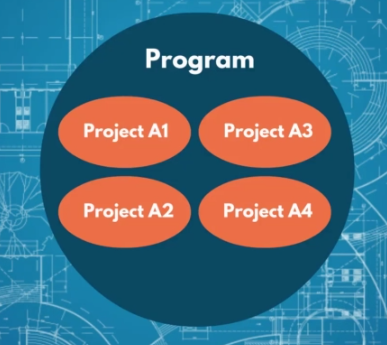
\includegraphics[width=\width\textwidth]{./figs/20221020221609.png}
            %\caption{}
        \end{figure}
    
    \item Portfolio management: The coordinated management of multiple programs and projects.
        \begin{figure}[H]
            \centering
            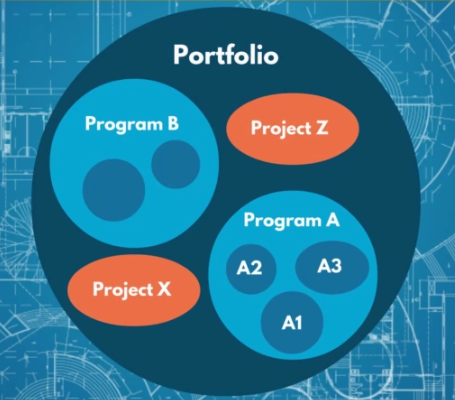
\includegraphics[width=\width\textwidth]{./figs/20221020221706.png}
            %\caption{}
        \end{figure}
        \begin{itemize}
            \item For example in a pharmaceutical company there might be several drugs being developed at the same time, this will be handled as diffrent project and inside a portfolio.
        \end{itemize}
\end{itemize}